\documentclass[11pt]{article}

\usepackage[a4paper,margin=1in]{geometry}
\usepackage{amsmath,amssymb,mathtools}
\usepackage{booktabs}
\usepackage{algorithm}
\usepackage{algpseudocode}
\usepackage{tikz}
\usetikzlibrary{arrows.meta,positioning,shapes}

\renewcommand{\Join}{\bowtie}
\newcommand{\Agg}[1]{\mathcal{L}_{#1}}
\renewcommand{\deg}{\operatorname{deg}}

\newcommand{\MATCH}{\textbf{match}}
\newcommand{\LET}{\textbf{let} \hspace{0.1em}}
\newcommand{\RETURN}{\textbf{return} \hspace{0.1em}}
\newcommand{\IF}{\textbf{if} \hspace{0.1em}}
\newcommand{\ELSE}{\textbf{else} \hspace{0.1em}}
\newcommand{\ENDIF}{\textbf{end if}\hspace{0.1em}}
\newcommand{\TAB}{\hspace*{1.2em}}
\newcommand{\VIEW}[1]{#1} % or your existing \VIEW macro
\newcommand{\sch}{\mathsf{sch}}
% \newcommand{\VIEW}[2][]{\ifthenelse{\isempty{#1}}{\mathsf{#2}\xspace}{\mathsf{#2[\mathit{#1}]}\xspace}}


\title{A Cost Model for Ranking View Trees}
\author{}
\date{}

\begin{document}
\maketitle

\paragraph{Goal.}
Given a view tree $T$ and an update workload, compute a \emph{symbolic cost expression} $\mathrm{Score}(T)$ to rank competing view trees (different variable orders) for the same query.

\section{Cost Model}

When a base relation receives updates, the changes propagate upward through the view tree.
At each view along the update path, we compute the delta to that view.
Our cost model uses the sizes of these deltas as a proxy for the computational work required to maintain the views.

\paragraph{View definitions.}
In view trees, an internal view is defined by \emph{joining} its child views.
Optionally, the view may also perform an \emph{aggregation/marginalization} step.
Thus, a single view may involve:
(i) a join step that combines the affected child delta with the other child views, and
(ii) an optional aggregation step that groups the join result by the view's output keys.

\paragraph{Per-view cost.}
Consider a view $V$ with children $V_1,\ldots,V_k$.
When an update arrives, only one child view is affected; let this be child $V_j$ with delta $\delta V_j$.
We estimate the delta size for $V$ in two stages.

\begin{enumerate}
  \item \textbf{Join stage.}
  The view first joins the affected delta with the other child views on the join key $A$.
  The size of the intermediate delta after the join is estimated as
  \[
  C_{\mathrm{join}}
  \;=\;
  |\delta V_j|\cdot \prod_{i\neq j}\deg_{V_i}(*\mid A),
  \]
  where $\deg_{V_i}(*\mid A)$ is the average number of tuples in $V_i$ per distinct value of $A$
  (equivalently, the average fanout when probing $V_i$ by $A$).

  \item \textbf{Optional aggregation stage.}
  If $V$ aggregates away bound variables, we estimate the output delta size by
  \[
  C_{\mathrm{agg}}
  \;=\;
  \min\bigl(|\delta V|_{\mathrm{join}},\, |Dom(keys)|\bigr),
  \]
  where $|Dom(keys)|$ is a domain cap for the variables of $V$.
\end{enumerate}

The cost incurred at view $V$ is the sum of the join and aggregation costs:
\[
C_V \;=\; C_{\mathrm{join}} + C_{\mathrm{agg}}.
\]


\paragraph{Total cost.}
We evaluate a view tree under a workload by summing the per-view delta sizes induced by updates to all
base relations.
We assume that, over a fixed time window, each updatable relation $R$ receives a batch of updates $\delta R$
of size $U_R$. Some relations may be non-updatable (e.g., dimension tables), in which case $U_R=0$.

For each relation $R$ with $U_R>0$, we treat $U_R$ as the input delta size at the leaf of $R$ and propagate
this delta upward along the unique path to the root.
At each view on the path, estimate the cost $C_V$ using the rules above.
% The total cost is the sum of these per-view costs along the update path.

The total maintenance cost for processing the accumulated updates to all base relations is obtained by repeating this process for every updatable relation $R$ (with its corresponding $U_R$) and summing the per-view contributions along each update path.


The next section gives the formal algorithmic formulation that computes this total score symbolically.
The result is a symbolic expression in $\{U_R\}$, $\{\deg_V(*|A)\}$, and $\{Dom(keys)\}$.



\paragraph{Algorithm.}
\begin{figure}[t]
\centering
\setlength{\tabcolsep}{3pt}
%
\begin{tabular}{@{}c@{}c@{~~~~}l@{}}
    \toprule
    \multicolumn{3}{c}{$\textsc{Score}(\text{view tree } \tau, \text{update } \VIEW{\delta R}) : (\Delta,\,S)$}\\
    \midrule
    \multicolumn{3}{l}{\MATCH \, $\tau$:}\\
    \midrule
    \phantom{a} & $R[\sch(R)]$ &
    \hspace*{0.5em}\RETURN $\bigl(|\VIEW{\delta R}|,\;0\bigr)$\\[2pt]
    \cmidrule{2-3} \\[-6pt]
    &
    \begin{minipage}[t]{1.6cm}
        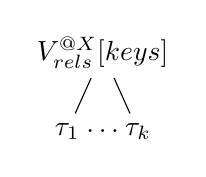
\begin{tikzpicture}[xscale=0.45, yscale=1]
            \node at (0,-2)  (n4) {$V^{@X}_{rels}[keys]$};
            \node at (-1,-3)  (n1) {$\tau_1$} edge[-] (n4);
            \node at (0,-3)  (n2) {$\ldots$};
            \node at (1,-3)  (n3) {$\tau_k$} edge[-] (n4);
        \end{tikzpicture}
    \end{minipage}
    &
    \begin{minipage}[t]{8.8cm}
\vspace{-4.4em}
  \hspace*{0.5em}\LET $V^{@X_i}_{rels_i}[keys_i]\text{ be root of } \tau_i,\ \forall i\in[k]$\\[0.5ex]
\hspace*{0.5em}\LET $j\in[k] \text{ be such that } \VIEW{R}\in\mathsf{rels}_j$ \\[0.5ex]
\hspace*{0.5em}\LET $(\Delta_j, S_j) \;=\; \textsc{Score}(\tau_j, \VIEW{\delta R})$ \\[0.7ex]


\hspace*{0.5em}\LET $\Delta_{\mathrm{join}} \;=\; \Delta_j \cdot \prod_{i\in[k],\,i\neq j}\deg_{{V^{@X_i}_{rels_i}}}(*\mid A)$ \\[0.7ex]

\hspace*{0.5em}\IF $X \notin keys$ \hfill{\small (aggregating / bound-variable node)}\\[0.5ex]
\TAB \LET $\Delta_{agg} \;=\; \min(\Delta_{\mathrm{join}},\, |Dom(keys)|)$ \\[0.5ex]
\TAB \RETURN $\bigl(\Delta_{agg},\; S_j + \Delta_{\mathrm{join}} + \Delta_{agg}\bigr)$ \\[0.7ex]

\hspace*{0.5em}\RETURN $\bigl(\Delta_{\mathrm{join}},\; S_j + \Delta_{\mathrm{join}}\bigr)$ \\[0.5ex]
    \end{minipage}
    \\
    \bottomrule
\end{tabular}
\caption{Recursive symbolic scoring.
Given a view tree $\tau$ and an update $\VIEW{\delta R}$ to base relation $\VIEW{R}$,
$\textsc{Score}(\tau,\VIEW{\delta R})$ returns: (i) $\Delta$, the estimated delta size at the root of $\tau$,
and (ii) $S$, the accumulated score along the unique update path (sum of per-view costs).
$F_{v\mid j}$ is the product of sibling fanouts (average degrees on join key $A$) when the delta comes from child $j$.
If the root variable $X$ is bound ($X\notin keys$), we apply the domain/NDV cap $D_v$ and charge both join and
aggregation work via $C_v=\Delta_{\mathrm{join}}+\Delta$; otherwise $C_v=\Delta$.}
\label{fig:score_recursive_paperstyle}
\end{figure}
 
The output is a symbolic expression in $\{U_R\}$, $\{\deg_V(*|A)\}$, $Dom(keys)$.

\section{Statistics}

The cost model requires three statistics: update volume $U_R$, join degree $\deg_V(*|A)$, and aggregation domain size $|Dom(keys)|$.

\paragraph{Update volume ($U_R$).}
$U_R$ is the number of update tuples accumulated for relation $R$ between consecutive maintenance rounds (i.e., the batch size).
Different relations exhibit different update frequencies; e.g., in TPC-H, \texttt{lineitem} and \texttt{orders} are high-frequency while \texttt{customer} and \texttt{nation} are low-frequency.
Obtain from historical measurement or workload specification.

\paragraph{Join degree ($\deg_V(*|A)$).}
$\deg_V(*|A)$ is the average number of tuples in view $V$ per distinct value of key $A$.
When a delta probes sibling view $V$ on join key $A$, each probe tuple finds $\deg_V(*|A)$ matches on average.

To estimate, use the view size and domain size:
$\deg_V(*|A) \approx |V| / |\mathrm{Dom}(A \text{ in } V)|$.
If $A$ is a primary key in $V$, then $\deg_V(*|A) = 1$.

Alternatively, if $V$ is indexed by $A$, $\deg_V(*|A)$ is the average bucket size.
Can also be measured at runtime.

\paragraph{Aggregation domain size ($D_v$).}
At an aggregation node $v$, the output delta size is bounded by the number of distinct group-by keys.
$D_v = |\mathrm{Dom}(\text{group-by keys})|$ at node $v$.
Obtain from catalog statistics, view size, or runtime measurement.

\paragraph{Stationarity assumption.}
The cost model uses current statistics to predict future maintenance costs, assuming statistics are approximately stationary: update frequencies $U_R$ remain stable, join degrees do not change drastically, and aggregation domains $D_v$ do not grow or shrink significantly.
When violated (e.g., data drift), re-calibrate by refreshing statistics periodically.

\section{Example: TPC-H Q10}

We consider TPC-H Q10 over the four relations:
$N=\textsf{nation}$, $C=\textsf{customer}$, $O=\textsf{orders}$, $L=\textsf{lineitem}$.
Let $U_R$ denote the (effective) batch size of updates to relation $R$ in one round
(predicate-conditioned, after applying query predicates).


%%%%%%%%%%%%%%%%%%%%%%%%%%%%%%%%%%%%%%%%%%%%%%%%%%%%%%%%%%%%%%%%%%%%%%%%%%%%%%
% vo1: orderkey -> custkey -> nationkey
%%%%%%%%%%%%%%%%%%%%%%%%%%%%%%%%%%%%%%%%%%%%%%%%%%%%%%%%%%%%%%%%%%%%%%%%%%%%%%
\subsection{vo1: $\texttt{orderkey} \rightarrow \texttt{custkey} \rightarrow \texttt{nationkey}$}

\begin{figure}[ht]
\centering
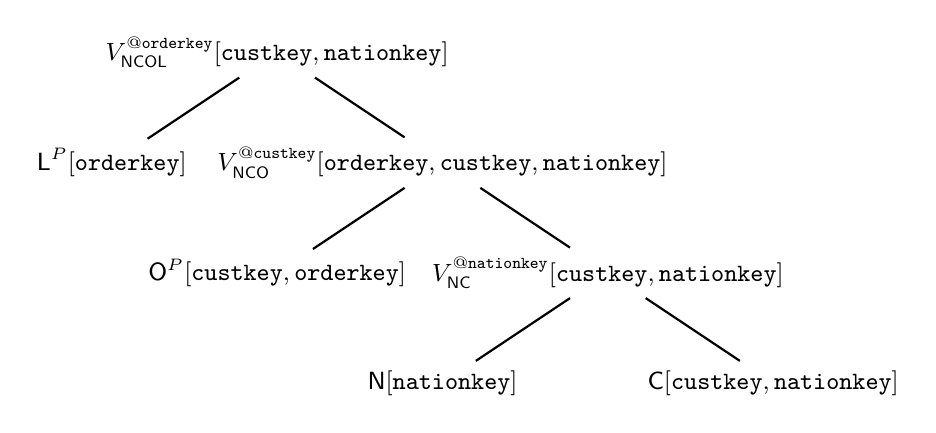
\begin{tikzpicture}[
  level distance=14mm,
  sibling distance=42mm,
  every node/.style={font=\small, align=center},
  edge from parent/.style={draw, thick}
]
\node (Vo)
{$V^{@\texttt{orderkey}}_{\textsf{NCOL}}[\texttt{custkey},\texttt{nationkey}]$}
  child { node (L)
    {$\textsf{L}^{P}[\texttt{orderkey}]$}
  }
  child { node (Vc)
    {$V^{@\texttt{custkey}}_{\textsf{NCO}}[\texttt{orderkey},\texttt{custkey},\texttt{nationkey}]$}
      child { node (O)
        {$\textsf{O}^{P}[\texttt{custkey},\texttt{orderkey}]$}
      }
      child { node (Vn)
        {$V^{@\texttt{nationkey}}_{\textsf{NC}}[\texttt{custkey},\texttt{nationkey}]$}
          child { node (N)
            {$\textsf{N}[\texttt{nationkey}]$}
          }
          child { node (C)
            {$\textsf{C}[\texttt{custkey},\texttt{nationkey}]$}
          }
      }
  };
\end{tikzpicture}
\caption{View tree vo1. The root $\texttt{orderkey}$-node is an aggregation node.}
\label{fig:vo1}
\end{figure}

\paragraph{Symbolic cost.}
Aggregation at root; N and C traverse 3 hops to reach it.
\begin{align*}
S_L &= \delta^{\mathrm{join}}_L + \delta^{\mathrm{agg}}_L,
\quad \delta^{\mathrm{join}}_L = U_L \cdot \deg_{V_{NCO}}(*|\texttt{okey}),\\[4pt]
S_O &= \delta_O + \delta^{\mathrm{join}}_O + \delta^{\mathrm{agg}}_O,
\quad \delta_O = U_O \cdot \deg_{V_{NC}}(*|\texttt{ckey}),\;
\delta^{\mathrm{join}}_O = \delta_O \cdot \deg_{L^P}(*|\texttt{okey}),\\[4pt]
S_C &= \delta^{(1)}_C + \delta^{(2)}_C + \delta^{\mathrm{join}}_C + \delta^{\mathrm{agg}}_C,\\
&\quad \delta^{(1)}_C = U_C \cdot \deg_N(*|\texttt{nkey}),\;
\delta^{(2)}_C = \delta^{(1)}_C \cdot \deg_{O^P}(*|\texttt{ckey}),\;
\delta^{\mathrm{join}}_C = \delta^{(2)}_C \cdot \deg_{L^P}(*|\texttt{okey}),\\[4pt]
S_N &= \delta^{(1)}_N + \delta^{(2)}_N + \delta^{\mathrm{join}}_N + \delta^{\mathrm{agg}}_N,\\
&\quad \delta^{(1)}_N = U_N \cdot \deg_C(*|\texttt{nkey}),\;
\delta^{(2)}_N = \delta^{(1)}_N \cdot \deg_{O^P}(*|\texttt{ckey}),\;
\delta^{\mathrm{join}}_N = \delta^{(2)}_N \cdot \deg_{L^P}(*|\texttt{okey}).
\end{align*}
All $\delta^{\mathrm{agg}} = \min(\delta^{\mathrm{join}}, |\mathrm{Dom}(\texttt{okey})|)$.
\[
\boxed{\mathrm{Score}_{\mathrm{vo1}} = S_N + S_C + S_O + S_L}
\]

\paragraph{Statistics (TPC-H SF=1).}
We compare statistics with and without query predicates
($O^P$: \texttt{o\_orderdate} $\in$ [1993-10-01, 1994-01-01);
$L^P$: \texttt{l\_returnflag} = 'R').

\smallskip
\noindent\textbf{Update batch sizes} (per 10000-tuple global batch, distributed by table size).
\begin{center}
\begin{tabular}{lrrl}
\toprule
& With Predicates & No Predicates & Note \\
\midrule
$U_N$ & 0 or 1 & 0 or 1 & (scenario-dependent) \\
$U_C$ & 196 & 196 & no predicate on $C$ \\
$U_O$ & 75 & 1961 & selectivity 3.8\% \\
$U_L$ & 1933 & 7844 & selectivity 24.6\% \\
\bottomrule
\end{tabular}
\end{center}

\paragraph{Grounded scores.}

\smallskip
\noindent\textbf{Static scenario ($U_N = 0$).}
\begin{center}
\begin{tabular}{lrr}
\toprule
& With Predicates & No Predicates \\
\midrule
$S_N$ & 0 & 0 \\
$S_C$ & 570 & 17843 \\
$S_O$ & 374 & 17647 \\
$S_L$ & 294 & 15687 \\
\midrule
\textbf{Total} & \textbf{1238} & \textbf{51178} \\
\bottomrule
\end{tabular}
\end{center}

\smallskip
\noindent\textbf{Dynamic scenario ($U_N = 1$).}
Nation updates are expensive (3-hop path to root).
\begin{center}
\begin{tabular}{lrr}
\toprule
& With Predicates & No Predicates \\
\midrule
$S_N$ & 17460 & 546097 \\
$S_C$ & 570 & 17843 \\
$S_O$ & 374 & 17647 \\
$S_L$ & 294 & 15687 \\
\midrule
\textbf{Total} & \textbf{18698} & \textbf{597275} \\
\bottomrule
\end{tabular}
\end{center}

%%%%%%%%%%%%%%%%%%%%%%%%%%%%%%%%%%%%%%%%%%%%%%%%%%%%%%%%%%%%%%%%%%%%%%%%%%%%%%
% vo2: orderkey -> nationkey -> custkey
%%%%%%%%%%%%%%%%%%%%%%%%%%%%%%%%%%%%%%%%%%%%%%%%%%%%%%%%%%%%%%%%%%%%%%%%%%%%%%
\subsection{vo2: $\texttt{orderkey} \rightarrow \texttt{nationkey} \rightarrow \texttt{custkey}$}

\begin{figure}[ht]
\centering
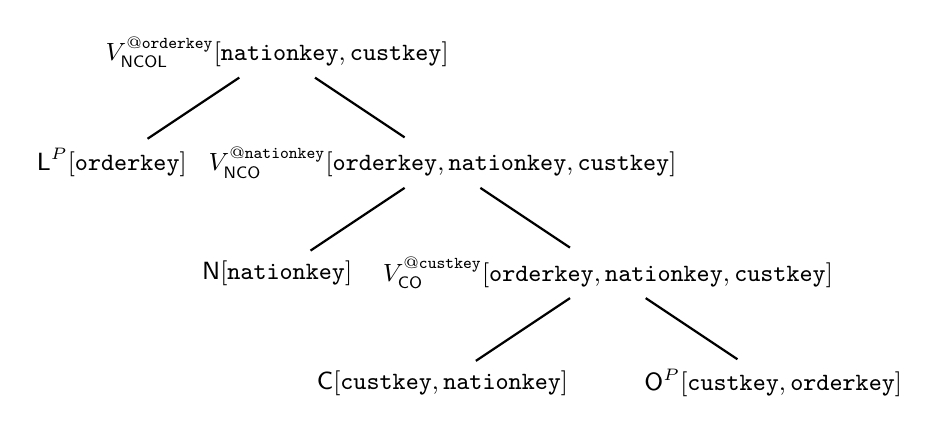
\begin{tikzpicture}[
  level distance=14mm,
  sibling distance=42mm,
  every node/.style={font=\small, align=center},
  edge from parent/.style={draw, thick}
]
\node (Vo)
{$V^{@\texttt{orderkey}}_{\textsf{NCOL}}[\texttt{nationkey},\texttt{custkey}]$}
  child { node (L)
    {$\textsf{L}^{P}[\texttt{orderkey}]$}
  }
  child { node (Vn)
    {$V^{@\texttt{nationkey}}_{\textsf{NCO}}[\texttt{orderkey},\texttt{nationkey},\texttt{custkey}]$}
      child { node (N)
        {$\textsf{N}[\texttt{nationkey}]$}
      }
      child { node (Vc)
        {$V^{@\texttt{custkey}}_{\textsf{CO}}[\texttt{orderkey},\texttt{nationkey},\texttt{custkey}]$}
          child { node (C)
            {$\textsf{C}[\texttt{custkey},\texttt{nationkey}]$}
          }
          child { node (O)
            {$\textsf{O}^{P}[\texttt{custkey},\texttt{orderkey}]$}
          }
      }
  };
\end{tikzpicture}
\caption{View tree vo2. The root $\texttt{orderkey}$-node is an aggregation node.}
\label{fig:vo2}
\end{figure}

\paragraph{Symbolic cost.}
Aggregation at root; N is at depth 2, C and O at depth 3.
\begin{align*}
S_L &= \delta^{\mathrm{join}}_L + \delta^{\mathrm{agg}}_L,
\quad \delta^{\mathrm{join}}_L = U_L \cdot \deg_{V_{NCO}}(*|\texttt{okey}),\\[4pt]
S_N &= \delta_N + \delta^{\mathrm{join}}_N + \delta^{\mathrm{agg}}_N,
\quad \delta_N = U_N \cdot \deg_{V_{CO}}(*|\texttt{nkey}),\;
\delta^{\mathrm{join}}_N = \delta_N \cdot \deg_{L^P}(*|\texttt{okey}),\\[4pt]
S_C &= \delta^{(1)}_C + \delta^{(2)}_C + \delta^{\mathrm{join}}_C + \delta^{\mathrm{agg}}_C,\\
&\quad \delta^{(1)}_C = U_C \cdot \deg_{O^P}(*|\texttt{ckey}),\;
\delta^{(2)}_C = \delta^{(1)}_C \cdot \deg_N(*|\texttt{nkey}),\;
\delta^{\mathrm{join}}_C = \delta^{(2)}_C \cdot \deg_{L^P}(*|\texttt{okey}),\\[4pt]
S_O &= \delta^{(1)}_O + \delta^{(2)}_O + \delta^{\mathrm{join}}_O + \delta^{\mathrm{agg}}_O,\\
&\quad \delta^{(1)}_O = U_O \cdot \deg_C(*|\texttt{ckey}),\;
\delta^{(2)}_O = \delta^{(1)}_O \cdot \deg_N(*|\texttt{nkey}),\;
\delta^{\mathrm{join}}_O = \delta^{(2)}_O \cdot \deg_{L^P}(*|\texttt{okey}).
\end{align*}
All $\delta^{\mathrm{agg}} = \min(\delta^{\mathrm{join}}, |\mathrm{Dom}(\texttt{okey})|)$.
\[
\boxed{\mathrm{Score}_{\mathrm{vo2}} = S_N + S_C + S_O + S_L}
\]

\paragraph{Grounded scores.}

\smallskip
\noindent\textbf{Static scenario ($U_N = 0$).}
\begin{center}
\begin{tabular}{lrr}
\toprule
& With Predicates & No Predicates \\
\midrule
$S_N$ & 0 & 0 \\
$S_C$ & 449 & 19608 \\
$S_O$ & 449 & 19608 \\
$S_L$ & 294 & 15687 \\
\midrule
\textbf{Total} & \textbf{1192} & \textbf{54903} \\
\bottomrule
\end{tabular}
\end{center}

\smallskip
\noindent\textbf{Dynamic scenario ($U_N = 1$).}
Nation updates are cheaper than vo1 (2-hop vs.\ 3-hop path).
\begin{center}
\begin{tabular}{lrr}
\toprule
& With Predicates & No Predicates \\
\midrule
$S_N$ & 11459 & 540097 \\
$S_C$ & 449 & 19608 \\
$S_O$ & 449 & 19608 \\
$S_L$ & 294 & 15687 \\
\midrule
\textbf{Total} & \textbf{12651} & \textbf{595000} \\
\bottomrule
\end{tabular}
\end{center}

%%%%%%%%%%%%%%%%%%%%%%%%%%%%%%%%%%%%%%%%%%%%%%%%%%%%%%%%%%%%%%%%%%%%%%%%%%%%%%
% vo3: nationkey -> custkey -> orderkey
%%%%%%%%%%%%%%%%%%%%%%%%%%%%%%%%%%%%%%%%%%%%%%%%%%%%%%%%%%%%%%%%%%%%%%%%%%%%%%
\subsection{vo3: $\texttt{nationkey} \rightarrow \texttt{custkey} \rightarrow \texttt{orderkey}$}

\begin{figure}[ht]
\centering
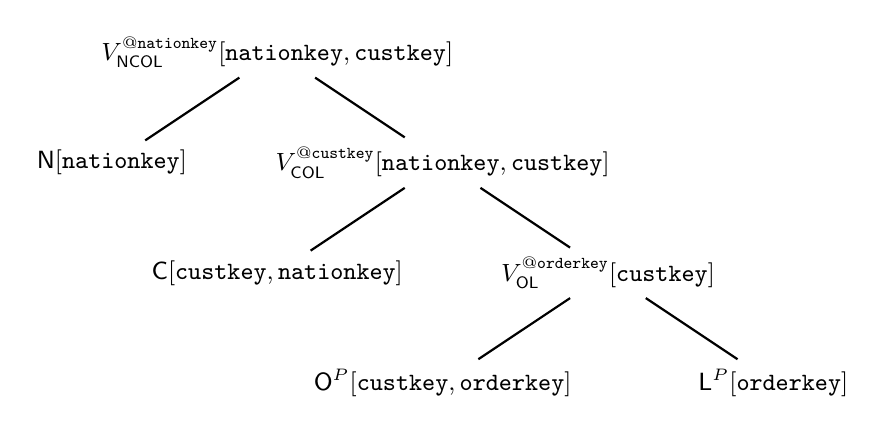
\begin{tikzpicture}[
  level distance=14mm,
  sibling distance=42mm,
  every node/.style={font=\small, align=center},
  edge from parent/.style={draw, thick}
]
\node (Vn)
{$V^{@\texttt{nationkey}}_{\textsf{NCOL}}[\texttt{nationkey},\texttt{custkey}]$}
  child { node (N)
    {$\textsf{N}[\texttt{nationkey}]$}
  }
  child { node (Vc)
    {$V^{@\texttt{custkey}}_{\textsf{COL}}[\texttt{nationkey},\texttt{custkey}]$}
      child { node (C)
        {$\textsf{C}[\texttt{custkey},\texttt{nationkey}]$}
      }
      child { node (Vo)
        {$V^{@\texttt{orderkey}}_{\textsf{OL}}[\texttt{custkey}]$}
          child { node (O)
            {$\textsf{O}^{P}[\texttt{custkey},\texttt{orderkey}]$}
          }
          child { node (L)
            {$\textsf{L}^{P}[\texttt{orderkey}]$}
          }
      }
  };
\end{tikzpicture}
\caption{View tree vo3. The $\texttt{orderkey}$-node is an aggregation node with output key \texttt{custkey}.}
\label{fig:vo3}
\end{figure}

\paragraph{Symbolic cost.}
\begin{align*}
S_N &= U_N \cdot \deg_{V_{COL}}(*|\texttt{nkey}), \\[4pt]
S_C &= U_C \cdot \deg_{V_{OL}}(*|\texttt{ckey}) \cdot (1 + \deg_N(*|\texttt{nkey})), \\[4pt]
S_O &= (\delta^{\mathrm{join}}_O + \delta^{\mathrm{agg}}_O) \cdot (1 + \deg_C(*|\texttt{ckey}) \cdot (1 + \deg_N(*|\texttt{nkey}))),
\\
&\qquad \text{where } \delta^{\mathrm{join}}_O = U_O \cdot \deg_{L^P}(*|\texttt{okey}),\;
\delta^{\mathrm{agg}}_O = \min(\delta^{\mathrm{join}}_O,\, |\mathrm{Dom}(\texttt{ckey})|), \\[4pt]
S_L &= (\delta^{\mathrm{join}}_L + \delta^{\mathrm{agg}}_L) \cdot (1 + \deg_C(*|\texttt{ckey}) \cdot (1 + \deg_N(*|\texttt{nkey}))),
\\
&\qquad \text{where } \delta^{\mathrm{join}}_L = U_L \cdot \deg_{O^P}(*|\texttt{okey}),\;
\delta^{\mathrm{agg}}_L = \min(\delta^{\mathrm{join}}_L,\, |\mathrm{Dom}(\texttt{ckey})|).
\end{align*}
\[
\boxed{\mathrm{Score}_{\mathrm{vo3}} = S_N + S_C + S_O + S_L}
\]

\paragraph{Grounded scores.}

\smallskip
\noindent\textbf{Static scenario ($U_N = 0$).}
\begin{center}
\begin{tabular}{lrr}
\toprule
& With Predicates & No Predicates \\
\midrule
$S_N$ & 0 & 0 \\
$S_C$ & 99 & 261 \\
$S_O$ & 900 & 47061 \\
$S_L$ & 881 & 47061 \\
\midrule
\textbf{Total} & \textbf{1880} & \textbf{94383} \\
\bottomrule
\end{tabular}
\end{center}

\smallskip
\noindent\textbf{Dynamic scenario ($U_N = 1$).}
\begin{center}
\begin{tabular}{lrr}
\toprule
& With Predicates & No Predicates \\
\midrule
$S_N$ & 1519 & 6000 \\
$S_C$ & 99 & 261 \\
$S_O$ & 900 & 47061 \\
$S_L$ & 881 & 47061 \\
\midrule
\textbf{Total} & \textbf{3398} & \textbf{100383} \\
\bottomrule
\end{tabular}
\end{center}

\paragraph{Observations.}
\begin{itemize}
\item Without predicates, the cost is $\sim$50$\times$ higher due to larger update batch sizes and higher fanouts.
\item A single nation update adds significant cost due to the large degree $\deg_{V_{COL}}(*|\texttt{nkey})$
(each nation matches $\sim$1500--6000 customers).
\end{itemize}

%%%%%%%%%%%%%%%%%%%%%%%%%%%%%%%%%%%%%%%%%%%%%%%%%%%%%%%%%%%%%%%%%%%%%%%%%%%%%%
% vo4: nationkey -> orderkey -> custkey
%%%%%%%%%%%%%%%%%%%%%%%%%%%%%%%%%%%%%%%%%%%%%%%%%%%%%%%%%%%%%%%%%%%%%%%%%%%%%%
\subsection{vo4: $\texttt{nationkey} \rightarrow \texttt{orderkey} \rightarrow \texttt{custkey}$}

\begin{figure}[ht]
\centering
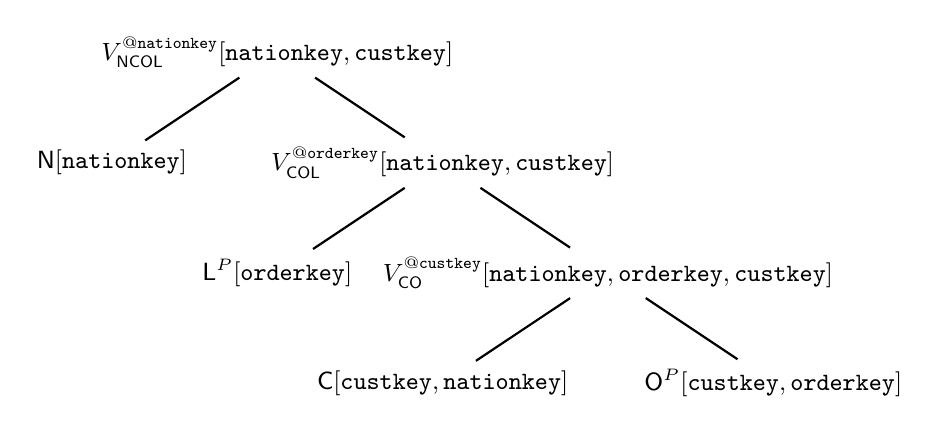
\begin{tikzpicture}[
  level distance=14mm,
  sibling distance=42mm,
  every node/.style={font=\small, align=center},
  edge from parent/.style={draw, thick}
]
\node (Vn)
{$V^{@\texttt{nationkey}}_{\textsf{NCOL}}[\texttt{nationkey},\texttt{custkey}]$}
  child { node (N)
    {$\textsf{N}[\texttt{nationkey}]$}
  }
  child { node (Vo)
    {$V^{@\texttt{orderkey}}_{\textsf{COL}}[\texttt{nationkey},\texttt{custkey}]$}
      child { node (L)
        {$\textsf{L}^{P}[\texttt{orderkey}]$}
      }
      child { node (Vc)
        {$V^{@\texttt{custkey}}_{\textsf{CO}}[\texttt{nationkey},\texttt{orderkey},\texttt{custkey}]$}
          child { node (C)
            {$\textsf{C}[\texttt{custkey},\texttt{nationkey}]$}
          }
          child { node (O)
            {$\textsf{O}^{P}[\texttt{custkey},\texttt{orderkey}]$}
          }
      }
  };
\end{tikzpicture}
\caption{View tree vo4. The $\texttt{orderkey}$-node is an aggregation node with output key \texttt{custkey}.}
\label{fig:vo4}
\end{figure}

\paragraph{Symbolic cost.}
\begin{align*}
S_N &= U_N \cdot \deg_{V_{COL}}(*|\texttt{nkey}), \\[4pt]
S_L &= (\delta^{\mathrm{join}}_L + \delta^{\mathrm{agg}}_L) \cdot (1 + \deg_N(*|\texttt{nkey})),
\quad \delta^{\mathrm{join}}_L = U_L \cdot \deg_{V_{CO}}(*|\texttt{okey}),\\[4pt]
S_C &= \delta_C + (\delta^{\mathrm{join}}_C + \delta^{\mathrm{agg}}_C) \cdot (1 + \deg_N(*|\texttt{nkey})),
\quad \delta_C = U_C \cdot \deg_{O^P}(*|\texttt{ckey}),\;
\delta^{\mathrm{join}}_C = \delta_C \cdot \deg_{L^P}(*|\texttt{okey}),\\[4pt]
S_O &= \delta_O + (\delta^{\mathrm{join}}_O + \delta^{\mathrm{agg}}_O) \cdot (1 + \deg_N(*|\texttt{nkey})),
\quad \delta_O = U_O \cdot \deg_C(*|\texttt{ckey}),\;
\delta^{\mathrm{join}}_O = \delta_O \cdot \deg_{L^P}(*|\texttt{okey}).
\end{align*}
All $\delta^{\mathrm{agg}} = \min(\delta^{\mathrm{join}}, |\mathrm{Dom}(\texttt{ckey})|)$.
\[
\boxed{\mathrm{Score}_{\mathrm{vo4}} = S_N + S_C + S_O + S_L}
\]

\paragraph{Grounded scores.}

\smallskip
\noindent\textbf{Static scenario ($U_N = 0$).}
\begin{center}
\begin{tabular}{lrr}
\toprule
& With Predicates & No Predicates \\
\midrule
$S_N$ & 0 & 0 \\
$S_C$ & 674 & 33334 \\
$S_O$ & 674 & 33334 \\
$S_L$ & 587 & 31374 \\
\midrule
\textbf{Total} & \textbf{1936} & \textbf{98042} \\
\bottomrule
\end{tabular}
\end{center}

\smallskip
\noindent\textbf{Dynamic scenario ($U_N = 1$).}
\begin{center}
\begin{tabular}{lrr}
\toprule
& With Predicates & No Predicates \\
\midrule
$S_N$ & 1519 & 6000 \\
$S_C$ & 674 & 33334 \\
$S_O$ & 674 & 33334 \\
$S_L$ & 587 & 31374 \\
\midrule
\textbf{Total} & \textbf{3454} & \textbf{104042} \\
\bottomrule
\end{tabular}
\end{center}

%%%%%%%%%%%%%%%%%%%%%%%%%%%%%%%%%%%%%%%%%%%%%%%%%%%%%%%%%%%%%%%%%%%%%%%%%%%%%%
% vo5: bushy (custkey root; children: nationkey and orderkey)
%%%%%%%%%%%%%%%%%%%%%%%%%%%%%%%%%%%%%%%%%%%%%%%%%%%%%%%%%%%%%%%%%%%%%%%%%%%%%%
\subsection{vo5: bushy (root \texttt{custkey}; children \texttt{nationkey}, \texttt{orderkey})}

\begin{figure}[ht]
\centering
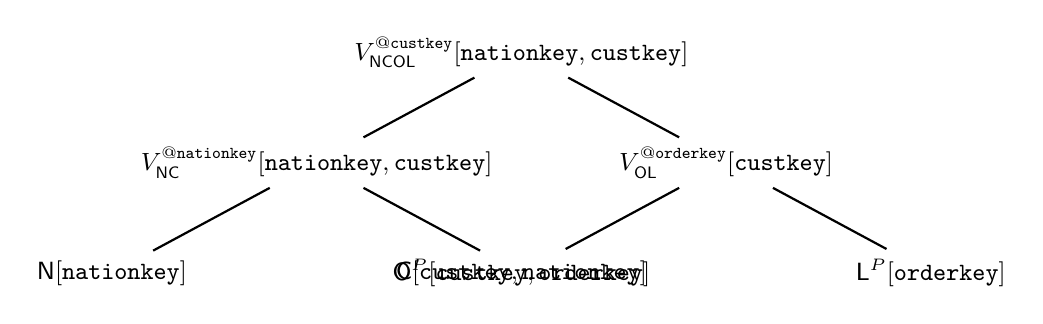
\begin{tikzpicture}[
  level distance=14mm,
  sibling distance=52mm,
  every node/.style={font=\small, align=center},
  edge from parent/.style={draw, thick}
]
\node (Vc)
{$V^{@\texttt{custkey}}_{\textsf{NCOL}}[\texttt{nationkey},\texttt{custkey}]$}
  child { node (Vn)
    {$V^{@\texttt{nationkey}}_{\textsf{NC}}[\texttt{nationkey},\texttt{custkey}]$}
      child { node (N)
        {$\textsf{N}[\texttt{nationkey}]$}
      }
      child { node (C)
        {$\textsf{C}[\texttt{custkey},\texttt{nationkey}]$}
      }
  }
  child { node (Vo)
    {$V^{@\texttt{orderkey}}_{\textsf{OL}}[\texttt{custkey}]$}
      child { node (O)
        {$\textsf{O}^{P}[\texttt{custkey},\texttt{orderkey}]$}
      }
      child { node (L)
        {$\textsf{L}^{P}[\texttt{orderkey}]$}
      }
  };
\end{tikzpicture}
\caption{View tree vo5 (bushy). The $\texttt{orderkey}$-node is an aggregation node.}
\label{fig:vo5}
\end{figure}

\paragraph{Symbolic cost.}
Bushy tree: N/C branch and O/L branch meet at the root.
\begin{align*}
S_C &= \delta_C \cdot (1 + \deg_{V_{OL}}(*|\texttt{ckey})),
\quad \delta_C = U_C \cdot \deg_N(*|\texttt{nkey}), \\[4pt]
S_N &= \delta_N \cdot (1 + \deg_{V_{OL}}(*|\texttt{ckey})),
\quad \delta_N = U_N \cdot \deg_C(*|\texttt{nkey}), \\[4pt]
S_O &= (\delta^{\mathrm{join}}_O + \delta^{\mathrm{agg}}_O) \cdot (1 + \deg_{V_{NC}}(*|\texttt{ckey})),
\quad \delta^{\mathrm{join}}_O = U_O \cdot \deg_{L^P}(*|\texttt{okey}),\\[4pt]
S_L &= (\delta^{\mathrm{join}}_L + \delta^{\mathrm{agg}}_L) \cdot (1 + \deg_{V_{NC}}(*|\texttt{ckey})),
\quad \delta^{\mathrm{join}}_L = U_L \cdot \deg_{O^P}(*|\texttt{okey}).
\end{align*}
$\delta^{\mathrm{agg}} = \min(\delta^{\mathrm{join}}, |\mathrm{Dom}(\texttt{ckey})|)$.
\[
\boxed{\mathrm{Score}_{\mathrm{vo5}} = S_N + S_C + S_O + S_L}
\]

\paragraph{Grounded scores.}

\smallskip
\noindent\textbf{Static scenario ($U_N = 0$).}
\begin{center}
\begin{tabular}{lrr}
\toprule
& With Predicates & No Predicates \\
\midrule
$S_N$ & 0 & 0 \\
$S_C$ & 246 & 327 \\
$S_O$ & 600 & 31374 \\
$S_L$ & 587 & 31374 \\
\midrule
\textbf{Total} & \textbf{1433} & \textbf{63074} \\
\bottomrule
\end{tabular}
\end{center}

\smallskip
\noindent\textbf{Dynamic scenario ($U_N = 1$).}
Nation updates are cheap (only 2-hop, no aggregation traversal).
\begin{center}
\begin{tabular}{lrr}
\toprule
& With Predicates & No Predicates \\
\midrule
$S_N$ & 7518 & 10000 \\
$S_C$ & 246 & 327 \\
$S_O$ & 600 & 31374 \\
$S_L$ & 587 & 31374 \\
\midrule
\textbf{Total} & \textbf{8951} & \textbf{73074} \\
\bottomrule
\end{tabular}
\end{center}

%%%%%%%%%%%%%%%%%%%%%%%%%%%%%%%%%%%%%%%%%%%%%%%%%%%%%%%%%%%%%%%%%%%%%%%%%%%%%%
% Summary
%%%%%%%%%%%%%%%%%%%%%%%%%%%%%%%%%%%%%%%%%%%%%%%%%%%%%%%%%%%%%%%%%%%%%%%%%%%%%%
\subsection{Summary and Rankings}

\paragraph{Cost comparison.}
\begin{center}
\begin{tabular}{lrrrr}
\toprule
& \multicolumn{2}{c}{With Predicates} & \multicolumn{2}{c}{No Predicates} \\
\cmidrule(lr){2-3} \cmidrule(lr){4-5}
VO & Static & Dynamic & Static & Dynamic \\
\midrule
vo1 & 1238 & 18698 & 51178 & 597275 \\
vo2 & 1192 & 12651 & 54903 & 595000 \\
vo3 & 1880 & 3398 & 94383 & 100383 \\
vo4 & 1936 & 3454 & 98042 & 104042 \\
vo5 & 1433 & 8951 & 63074 & 73074 \\
\bottomrule
\end{tabular}
\end{center}

\paragraph{Rankings by scenario.}

\smallskip
\noindent\textbf{Static scenario ($U_N = 0$): dimension tables not updated.}
\begin{center}
\begin{tabular}{clrclr}
\toprule
\multicolumn{3}{c}{With Predicates} & \multicolumn{3}{c}{No Predicates} \\
\cmidrule(lr){1-3} \cmidrule(lr){4-6}
Rank & VO & Score & Rank & VO & Score \\
\midrule
1 & vo2 & 1192 & 1 & vo1 & 51178 \\
2 & vo1 & 1238 & 2 & vo2 & 54903 \\
3 & vo5 & 1433 & 3 & vo5 & 63074 \\
4 & vo3 & 1880 & 4 & vo3 & 94383 \\
5 & vo4 & 1936 & 5 & vo4 & 98042 \\
\bottomrule
\end{tabular}
\end{center}

\smallskip
\noindent\textbf{Dynamic scenario ($U_N = 1$): dimension tables updated.}
\begin{center}
\begin{tabular}{clrclr}
\toprule
\multicolumn{3}{c}{With Predicates} & \multicolumn{3}{c}{No Predicates} \\
\cmidrule(lr){1-3} \cmidrule(lr){4-6}
Rank & VO & Score & Rank & VO & Score \\
\midrule
1 & vo3 & 3398 & 1 & vo5 & 73074 \\
2 & vo4 & 3454 & 2 & vo3 & 100383 \\
3 & vo5 & 8951 & 3 & vo4 & 104042 \\
4 & vo2 & 12651 & 4 & vo2 & 595000 \\
5 & vo1 & 18698 & 5 & vo1 & 597275 \\
\bottomrule
\end{tabular}
\end{center}

\paragraph{Key observations.}
\begin{itemize}
\item The optimal variable order depends critically on whether the nation table is updated:
  \begin{itemize}
  \item \textbf{Static nation:} vo1 and vo2 are best---placing the aggregation node at the root minimizes the path length for high-frequency O/L updates.
  \item \textbf{Dynamic nation:} vo3 and vo4 are best---placing nation near the root (depth 1) keeps $S_N$ small.
  \end{itemize}
\item vo1 and vo2 place nation at depth 3 and 2, respectively. A single nation update propagates through multiple joins, causing $S_N$ to explode (e.g., 18k vs.\ 3k for vo3 with predicates).
\item vo5 (bushy) provides a robust compromise: ranked 3rd in static scenarios and 1st--3rd in dynamic scenarios.
\item Predicates reduce total cost by $\sim$50$\times$ due to smaller effective batch sizes and lower join fanouts.
\end{itemize}


\end{document}
